\documentclass[../portafolio.tex]{subfiles}

% Solo agregue paquetes en el preámbulo de ../portafolio.tex

\begin{document}

\chapter{Instrucciones generales}
\label{ch:instrucciones}
%%%%%%%%%%%%%%%%%%%%%%%%%%%%%%%%%%%%%%%%%%%%%%%%%%%%%%%%%%%%%%%%%%%%%%%%%%%%%%%%

\hfill \textbf{Fecha de la actividad:} 10 de septiembre de 2024

\medskip

\textcolor{red}{\bf Elimine este capítulo de su portafolio}. Este
capítulo contiene algunas instrucciones generales de presentación de
su portafolio.

Las evidencias de aprendizaje en este portafolio consistirán en la
entrega de soluciones detalladas a problemas específicos seleccionados
durante la asignatura. Para cada evidencia, deberá incluir:

\begin{description}
\item[Fecha] La fecha en que empezó a escribir el capítulo.
\item[Resumen y objetivos] Explique claramente el problema que está resolviendo,
  especificando los objetivos del mismo y una descripción breve de
  cómo resolverá el problema. Note que esto \textbf{no se refiere al
    enunciado del problema de una guía}, sino que a un párrafo donde
  usted debe explicar qué es lo que quiere resolver.
\item[Método de solución] Describa cómo resuelve el problema. Por
  ejemplo, si tiene que demostrar algún esquema numérico, explique el
  procedimiento para tal demostración; y si va a resolver un problema,
  indique qué enfoque numérico o algoritmo usará para resolver el
  problema. En casos donde resuelva un problema de forma numérica,
  incluya detalles relevantes del código en \texttt{python},
  destacando aspectos importantes como la elección de esquemas
  numéricos, el uso de funciones, etc. \textbf{No incluya el código
    completo}, solo la parte más relevante para resolver el
  problema. Por ejemplo, puede omitir lineas donde importa librerías
  como \texttt{numpy} o \texttt{matplotlib}, o líneas donde está
  configurando un gráfico.

\item[Análisis de resultados] Presente y analice los resultados
  obtenidos. Por ejemplo, en un problema que involucre un esquema de
  derivadas centradas, discuta los errores numéricos encontrados y su
  comportamiento, mostrando gráficos o tablas, o citando referencias
  bibliográficas si es necesario.

\item[Conclusiones] Incluya un breve resumen (nuevamente) de lo que se
  hizo en la actividad y los resultados más importantes. Explique qué
  aprendió al resolver el problema, incluyendo cualquier dificultad
  que encontró y cómo la superó. También mencione cómo este problema
  contribuye a su comprensión de los métodos computacionales en
  física.

\item[Agradecimientos] Si aplica, incluya una breve reseña a las
  personas que lo ayudaron a resolver esta actividad.
\end{description}

En el capítulo \ref{ch:ejemplo-derivadas} mostramos un ejemplo de un problema simple ya resuelto en clases.


%---------------------------------------------------------------------------------
A continuación se presenta una breve guía de elementos que puede usar en \LaTeX\ para cuidar la presentación del mismo:
\section{Ecuaciones}

Dependiendo de su estilo, puede utilizar ecuaciones dentro del texto como
$f(x)=\frac{x}{\sqrt{1-x^2}}$.

\subsection{Ecuaciones largas}
Si la ecuación es larga o es importante (aunque no sea tan larga), debería dedicar una línea solo para esa ecuación. Así, para ecuaciones que son claramente relevantes, debe enumerarlas usando \texttt{equation}. Por ejemplo,
\begin{equation}
  \label{eq:euler}
\exp(i\theta) = \cos(\theta) + i\sin(\theta) \,.
\end{equation}

Si la ecuación es parte de un procedimiento, debe usar \texttt{align}. Por ejemplo,
\begin{align}
  \frac{d}{dx} x^2 \sin x
  &= \left(\frac{dx^2}{dx}\right)  \sin x + x^2 \frac{d}{dx} \sin x \,, \nonumber \\
  &= 2x \sin x + x^2 \cos x \,. \label{eq:regla-producto}
\end{align}

Note el uso de \verb@\nonumber@ para eliminar la enumeración de una
línea. Note también el uso de puntos y comas en las ecuaciones
\eqref{eq:euler} a \eqref{eq:regla-producto}.

\subsection{Referencia a ecuaciones}
Puede citar ecuaciones enumeradas, por ejemplo la ecuación de Euler
\eqref{eq:euler} es una de las ecuaciones básicas del cálculo
complejo. Note que usamos el comando \verb@\eqref{eq:euler}@ para citar esta
ecuación. Para ello, es necesario dar una etiqueta a la ecuación que
quiere citar, para lo cual debe usar \verb@\label@. Note que la
etiqueta debería tener un nombre explícito. Por ejemplo, usamos
\verb@\label{eq:euler}@ porque claramente nos queremos referir a la
ecuación de Euler. No tiene sentido que use un número explícito como
\verb@\label{eq:1}@ porque es muy posible que ese número cambie en el
futuro.

De la misma forma, note que podemos hacer referencias a ecuaciones de otros capítulos e, incluso, a un capítulo completo. Por ejemplo, en la sección \ref{ch:ejemplo-derivadas} mostraremos un ejemplo de la solución de un problema numérico.

\section{Figuras}
También puede agregar figuras para explicar mejor sus ideas. Trate de
citarlas adecuadamente en el texto, por ejemplo, la figura
\ref{fig:estatica} muestra un ejemplo usado en wikipedia
para explicar la electricidad estática~\cite{wikistatic}.
\begin{figure}[ht!]
  \centering
  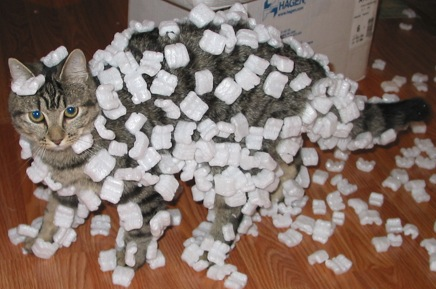
\includegraphics[width=0.5\textwidth]{static_cat_wikipedia}
  \caption{Bolas de poliestireno adheridos al pelaje de un gato debido
    a la electricidad estática.~\cite{wikistatic}.}
  \label{fig:estatica}
\end{figure}

En este caso, citamos la figura usando el comando \verb@\ref{fig:estatica}@. No es una buena práctica tratar de referirse a una figura como ``la siguiente figura'' porque estas tienden a moverse en el texto para aprovechar mejor los espacios. \textcolor{red}{\bf NO INTENTE FORZAR LA POSICIÓN DE UNA FIGURA}. O sea, \textbf{nunca} use \texttt{[H]} para que la figura aparezca donde usted quiere. Deje que la figura sea libre y que \LaTeX\ decida dónde queda mejor. Por ejemplo, es posible que la figura~\ref{fig:estatica} se encuentre en otra página en la compilación de este documento. Pero no importa, porque usted sabe que me estoy refiriendo a la figura~\ref{fig:estatica} y no a otra cosa.


\section{Códigos}
Puede incluir códigos usando el paquete \texttt{minted}. Esta librería
requiere que el compilador de \LaTeX\ se ejecute con
\texttt{-flag-escape} para procesar correctamente los colores del
código que usted incluya. Si tiene \LaTeX\ instalado localmente en su
computador, le recomiendo compilar con:
\begin{verbatim}
latexmk -pdf -shell-escape portafolio 
\end{verbatim}
%
Esto asegura la correcta compilación de todos los elementos del
documento, incluyendo referencias cruzadas a figuras y ecuaciones,
además de citas bibliográficas. La etiqueta \texttt{-pdf} es para
compilar el documento en formato PDF.

Para incluir código de python, use la siguiente sintaxis:
\begin{verbatim}
\begin{pythoncode}
   # código
\begin{pythoncode}
\end{verbatim}

Por ejemplo, la siguiente linea muestra cómo calcular la derivada centrada de una serie de puntos \texttt{(x[i],y[i])} usando un ciclo \texttt{for}:
\begin{pythoncode}
for i in range(1,y.size-1):
    dy[i] = (y[i+1]-y[i-1]) / (x[i+1]-x[i-1])
\end{pythoncode}

Para otro tipo de código, reemplace \texttt{pythoncode} por \texttt{minted}. Vea \href{https://www.overleaf.com/learn/latex/Code_Highlighting_with_minted}{la documentación de overleaf} para más ejemplos.


\section{Referencias bibliográficas}
Al final del documento encontrará una lista de referencias. Esto se logra usando \texttt{bibtex} y el archivo \texttt{referencias.bib} que se encuentra en el directorio base de este portafolio.

El archivo \texttt{referencias.bib} tiene entradas de la forma:
\begin{verbatim}
@misc{wikistatic,
    author = "{Wikipedia contributors}",
    title = "Static electricity --- {Wikipedia}{,} The Free Encyclopedia",
    year = "2021",
    howpublished = {\url{https://en.wikipedia.org/w/index.php?title=Static...}},
    note = "[Online; accessed 5-November-2021]"
  }
\end{verbatim}

En este caso, es una referencia a una página web y es de tipo \verb!@misc!, donde la primera palabra \texttt{wikistatic} es la etiqueta que usamos para citar, y las entradas \texttt{author}, \texttt{title}, etc. son información que \texttt{bibtex} usa para formatear la bibliografía al final del documento.

Para citar esta referencia en el texto, usamos el comando \verb@\citep{wikistatic}@. Puede citar más referencias separándolas con comas, por ejemplo \verb@\citep{wikistatic,AF:2003,CEL:arXiv}@ que resulta en \citep{wikistatic,AF:2003,CEL:arXiv}. Note que existen tres comandos disponibles \verb@\cite@, \verb@\citet@ y \verb@\citep@. Abajo explico un poco más.

Para compilar este documento (si es que está trabajando localmente en su computador con \LaTeX\ instalado), recomiendo usar el comando \texttt{latexmk}:
\begin{verbatim}
latexmk -pdf -shell-escape portafolio.tex
\end{verbatim}

Esto asegura la correcta compilación de todos los elementos del
documento, incluyendo referencias cruzadas a figuras y ecuaciones,
además de citas bibliográficas. La etiqueta \texttt{-pdf} es para compilar el documento en formato PDF, mientras que \texttt{-shell-escape} permite usar una librería para el formato de códigos de python insertos en \LaTeX.

Si tiene algún problema con la bibliografía, es posible que no tenga algunos elementos instalados (como la librería \texttt{texlive-publishers}). Busque en \texttt{portafolio.tex} la siguiente línea para diagnosticar el problema:
\begin{verbatim}
% % bibliografia: descomente estas dos lineas para usar estilo numerico, e.g. [1].
% \usepackage[square,numbers,sort&compress]{natbib}
% \bibliographystyle{apsrev4-1}

% bibliografia: descomente estas dos lineas para usar estilo autor-año, e.g. (Navarro, 2022).
\usepackage[authoryear]{natbib}
\bibliographystyle{aipauth4-1}

...

% lista de referencias guardadas en referencias.bib
\bibliography{referencias}

\end{document}
\end{verbatim}


En el texto anterior, \verb@\bibliographystyle@ controla el estilo de bibliografía. Por ejemplo,
\begin{itemize}
\item El estilo \texttt{apsrev4-1} configurado con \texttt{square,numbers,sort\&compress} resulta resulta en referencias numéricas:
\begin{verbatim}
\cite{CEL:arXiv}  : [3]
\citep{CEL:arXiv} : [3]
\citet{CEL:arXiv} : Cancès et al. [3]
\end{verbatim}

\item El estilo \texttt{aipauth4-1} configurado con \texttt{authoryear} resulta resulta en referencias autor-año:
\begin{verbatim}
\cite{CEL:arXiv}  : Cancès, Ehrlacher, and Lelièvre (2012)
\citep{CEL:arXiv} : (Cancès, Ehrlacher, and Lelièvre, 2012)
\citet{CEL:arXiv} : Cancès, Ehrlacher, and Lelièvre (2012)
\end{verbatim}
\end{itemize}


\section{Comentarios finales}

Note que este archivo se puede compilar independientemente del portafolio. Esto es posible gracias al paquete \texttt{subfiles}.

Al principio de este archivo, encuentra la instrucción
\begin{verbatim}
\documentclass[../portafolio.tex]{subfiles}
\end{verbatim}

Esto significa que este archivo hereda los paquetes y algunas configuraciones del archivo principal \texttt{../portafolio.tex}.

Para compilar este capítulo y solo este capítulo, puede usar:
\begin{verbatim}
latexmk -pdf -shell-escape template-instrucciones
\end{verbatim}

Es posible que las referencias bibliográficas no se resuelvan bien (puesto que no incluimos \verb@\bibliography{referencias}@ en este documento). Además, si cita ecuaciones o figuras de otros capítulos tampoco se resolverán, apareciendo un símbolo como (??). Pero esto no importa, pues la utilidad de esto es solo  compilar este documento de forma rápida para diagnosticar como se está viendo este. Una vez este capítulo esté finalizado, puede compilar el portafolio completo y las referencias estarán bien resueltas.
\end{document}
